
The first reaction many programmers have when they learn the material from the previous section is often this: "Thanks, I understand now why my program is slow, but I have to process the amount of data I have, not the ideal 32 KB, and the algorithm is what it is, including the complex data access pattern, so there is nothing I can do about it." This chapter would not be worth much if we didn't learn how to get better memory performance for the problems we need to solve. In this section, we will learn the techniques that can be used to improve memory performance.

\subsubsubsection{4.5.1\hspace{0.2cm}Memory-efficient data structures}

The choice of data structures, or, more generally, data organization, is usually the most important decision the programmer makes as far as memory performance is concerned. It is important to understand what you can and cannot do: the memory performance shown in Figure 4.5 and Figure 4.6 is really all there is, and you can't get around it (strictly speaking, this is only 99\% true; there are some exotic memory access techniques that, rarely, can exceed the limits shown in these figures). But, you can choose where on these graphs is the point corresponding to your program. Let us consider first a simple example: we have 1 M 64-bit integers that we need to store and process in order. We can store these values in an array; the size of the array will be 8 MB, and, according to our measurements, the access time is about 0.6 nanoseconds per value, as shown in Figure 4.6.

\hspace*{\fill} \\ %插入空行
\begin{center}
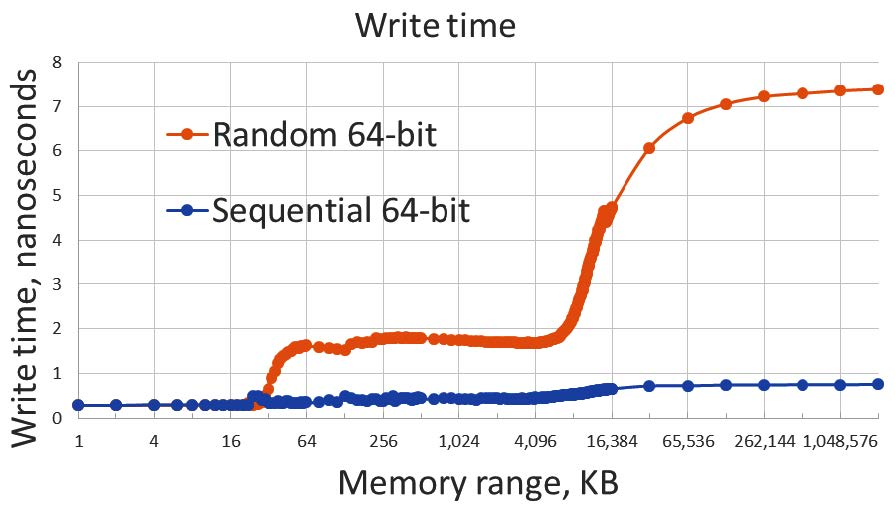
\includegraphics[width=0.9\textwidth]{content/1/chapter4/images/9.jpg}\\
Figure 4.9 – Write time for one array (A) versus list (L) element
\end{center}

Alternatively, we could use a list to store the same numbers. The std::list is a collection of nodes, and each node has the value and two pointers to the next and the previous node. The entire list, therefore, uses 24 MB of memory. Furthermore, each node is allocated through a separate call to operator new, so different nodes are likely to be at very different addresses, especially if the program is doing other memory allocations and deallocations at the same time. There isn't going to be any pattern in the addresses we need to access when traversing the list, so to find the performance of the list, all we need to do is find the point corresponding to the 24 MB memory range on the curve for random memory accesses. This gives us just over 5 nanoseconds per value or almost an order of magnitude slower than accessing the same data in an array.

Those of you who, at this point, demanded proof, have learned something valuable from the previous chapter. We can easily construct a micro-benchmark to compare writing data into a list and a vector of the same size. Here is the benchmark for the vector:

\hspace*{\fill} \\ %插入空行
\noindent
\textbf{03\_list\_vector.C}
\begin{lstlisting}[style=styleCXX]
template <class Word>
void BM_write_vector(benchmark::State& state) {
	const size_t size = state.range(0);
	std::vector<Word> c(size);
	Word x = {};
	for (auto _ : state) {
		for (auto it = c.begin(), it0 = c.end(); it !=
		it0;) {
			REPEAT(benchmark::DoNotOptimize(*it++ = x);)
		}
		benchmark::ClobberMemory();
	}
}
BENCHMARK_TEMPLATE1(BM_write_vector, unsigned long)-
>Arg(1<<20);
\end{lstlisting}

Change std::vector to std::list to create a list benchmark. Note that the meaning of the size has changed, compared to the earlier benchmarks: now it is the number of the elements in the container, so the memory size will depend on the element type and the container itself, just as was shown in Figure 4.6. The results, for 1 M elements, are exactly as promised:

\hspace*{\fill} \\ %插入空行
\begin{center}
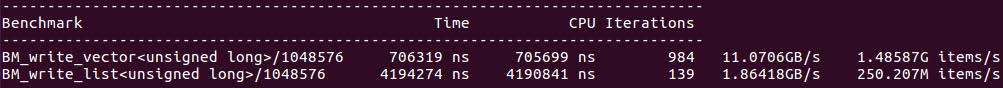
\includegraphics[width=0.9\textwidth]{content/1/chapter4/images/10.jpg}\\
Figure 4.10 – List versus vector benchmark
\end{center}

Why would anyone choose the list over the array (or std::vector)? The most common reason is that at the time of creation, we did not know how much data we were going to have, and growing a vector is extremely inefficient because of the copying involved. There are several ways around this problem. Sometimes it is possible to precompute the final size of the data relatively inexpensively. For example, it may cost us a single scan of the input data to determine how much space to allocate for the results. If the inputs are efficiently organized, it may be worth it to do two passes over the inputs: first, to count, and second, to process.

If it is not possible to know the final data size in advance, we may need a smarter data structure that combines the memory efficiency of a vector with the resizing efficiency of a list. This can be achieved using a block-allocated array:

\hspace*{\fill} \\ %插入空行
\begin{center}
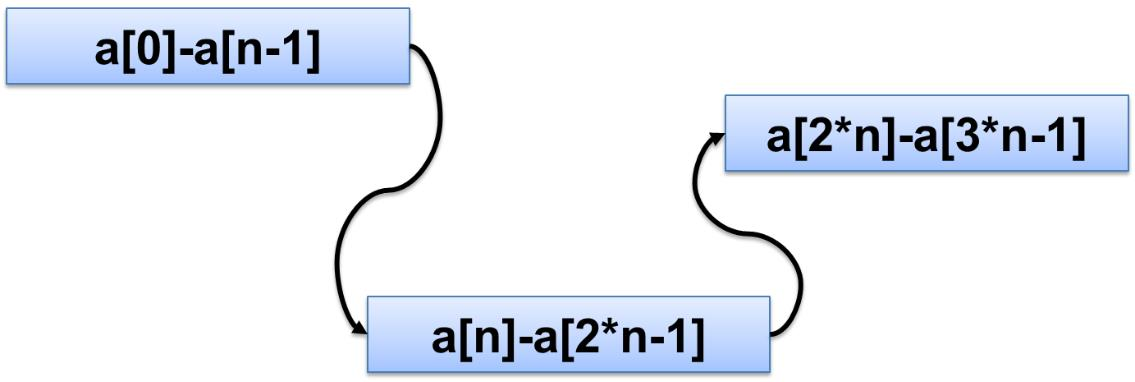
\includegraphics[width=0.9\textwidth]{content/1/chapter4/images/11.jpg}\\
Figure 4.11 – A block-allocated array (deque) can be grown in place
\end{center}

This data structure allocates memory in blocks of a fixed amount, usually small enough that they fit into the L1 cache (anywhere between 2 KB and 16 KB is commonly used). Each block is used as an array, so, within each block, the elements are accessed sequentially. The blocks themselves are organized in a list. If we need to grow this data structure, we just allocate another block and add it to the list. Accessing the first element of each block is likely to incur a cache miss, but the rest of the elements in the block can be accessed efficiently once the prefetch detects the pattern of sequential access. Amortized over the number of elements in each block, the cost of the random access can be made very small, and the resulting data structure can perform almost identically to the array or vector. In STL, we have such a data structure: std::deque (unfortunately, the implementation in most STL versions is not particularly efficient, and sequential accesses to the deque are usually somewhat slower than to the vector of the same size).

Yet another reason to prefer a list over an array, monolithic or block-allocated, is that the list allows fast insertions at any point, not just at the ends. If you need this, then you have to use a list or another node-allocated container. In such cases, often the best solution is to not attempt to select a single data structure that works for all requirements but to migrate the data from one data structure to another. For example, if we want to use the list to store data elements, one at a time while maintaining sorted order, one question to ask is, do we need the order to be sorted at all times, only after all elements are inserted, or a few times in the middle of the construction process but not all the time?

If there is a point in the algorithm where the data access patterns change, it is often advantageous to change the data structure at that point, even at the cost of some copying of memory. For example, we may construct a list and, after the last element is added, copy it into an array for faster sequential access (assuming we won't need to add any more elements). If we can be sure that some part of the data is complete, we may convert that part to an array, perhaps one or more blocks in a block-allocated array, and leave the still mutable data in a list or a tree data structure. On the other hand, if we rarely need to process the data in the sorted order, or need to process it in multiple orders, then separating the order from the storage is often the best solution. The data is stored in a vector or a deque, and the order is imposed on top of it by an array of pointerssorted in the desired order.  Since all ordered data accesses are now indirect (through an intermediate pointer), this is efficient only if such accesses are rare, and most of the time, we can process the data in the order in which it's stored in the array.

The bottom line is, if we access some data a lot, we should choose a data structure that makes that particular access pattern optimal. If the access pattern changes in time, the data structure should change as well. On the other hand, if we don't spend much time accessing the data, the overhead of converting from one arrangement of the data to another likely cannot be justified. However, in this case, inefficient data access should not be a problem in the first place. This brings us to the next question: how do we figure out which data is accessed inefficiently and, more generally, which data is expensive to access?

\subsubsubsection{4.5.2\hspace{0.2cm}Profiling memory performance}

Often, the efficiency of a particular data structure or data organization is fairly obvious. For example, if we have a class containing an array or a vector, and the interface of this class allows only one mode of access to the data, with sequential iteration from the beginning to the end (forward iterator, in the STL language), then we can be quite certain that the data is accessed as efficiently as possible, at the memory level anyway. We can't be sure about the efficiency of the algorithm: for example, a linear search of a particular element in an array is very inefficient (each memory read is efficient, of course, but there are a lot of them; we know better ways to organize data for searching).

Simply knowing which data structures are memory-efficient is not enough: we also need to know how much time the program spends working on a particular set of data. Sometimes, this is self-evident, especially with good encapsulation. If we have a function that, according to the profile or the timing report, takes a lot of time, and the code inside the function is not particularly heavy on computations but moves a lot of data, the odds are good that making access to this data more efficient will improve the overall performance.

Unfortunately, that is the easy case, and so it gets optimized first. Then we get to the point where no single function or code fragment stands out in terms of execution time, but the program is still inefficient. When you have no hot code, very often you have hot data: one or more data structures that are accessed throughout the program; the cumulative time spent on this data is large, but it's not localized to any function or loop. Conventional profiling does not help us: it will show that the runtime is spread evenly across the entire program, and optimizing any one fragment of code will yield very little improvement. What we need is a way to find the data that is accessed inefficiently throughout the program, and it adds up.

It is very hard to collect this information with just time-measuring tools. However, it can be collected fairly easily using a profiler that utilizes the hardware event counters. Most CPUs can count memory accesses and, more specifically, cache hits and misses. In this chapter, we again use the perf profiler; with it, we can measure how effective the L1 cache is used with this command:

\begin{tcblisting}{commandshell={}}
$ perf stat -e \
  cycles,instructions,L1-dcache-load-misses,L1-dcache-loads \
  ./program
\end{tcblisting}

The cache measurement counters are not part of the default counter set and must be specified explicitly. The exact set of available counters varies from one CPU to another but can always be viewed by running the perf list command. In our example, we measure L1 cache misses when reading data. The term dcache stands for data cache (pronounced dee-cache); the CPUs also have a separate instruction cache or icache (pronounced ay-cache) that is used to load the instructions from memory.

We can use this command line to profile our memory benchmarks for reading the memory at random addresses. When the memory range is small, say, 16 KB, the entire array fits into the L1 cache, and there are almost no cache misses:

\hspace*{\fill} \\ %插入空行
\begin{center}
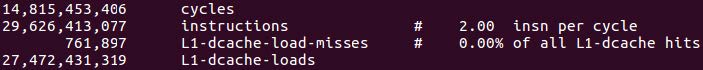
\includegraphics[width=0.9\textwidth]{content/1/chapter4/images/12.jpg}\\
Figure 4.12 – Profile of a program with good use of the L1 cache
\end{center}

Increasing the memory size to 128 MB means that cache misses are very frequent:

\hspace*{\fill} \\ %插入空行
\begin{center}
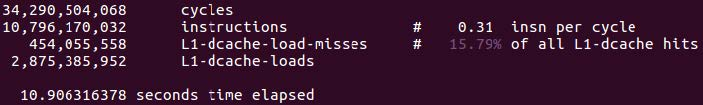
\includegraphics[width=0.9\textwidth]{content/1/chapter4/images/13.jpg}\\
Figure 4.13 – Profile of a program with poor use of the L1 cache
\end{center}

Note that perf stat collects the overall values for the entire program, where some memory accesses are cache-efficient, and others aren't. Once we know that somebody, somewhere, is handling memory accesses badly, we can get a detailed profile using perf record and perf report, as was shown in Chapter 2, Performance Measurements (we used a different counter there, but the process is the same for any counter we choose to collect). Of course, if our original timing profile failed to detect any hot code, the cache profile will show the same. There will be many locations in the code where the fraction of cache misses is large. Each location contributes only a small amount of time to the overall execution time, but it adds up. It is now up to us to notice that many of these code locations have one thing in common: the memory they operate on. For example, if we see that there are dozens of different functions that, between them all, account for the 15\% cache miss rate, but they all operate on the same list, then the list is the problematic data structure, and we have to organize our data in some other way.

We have now learned how to detect and identify the data structures whose inefficient memory access patterns negatively impact performance and what are some of the alternatives. Unfortunately, the alternative data structures usually don't have the same features or performance: a list cannot be replaced with a vector if elements must be inserted at arbitrary locations throughout the life of the data structure. Often, it is not the data structure but the algorithm itself that calls for inefficient memory accesses. In such cases, we may have to change the algorithms.

\subsubsubsection{4.5.3\hspace{0.2cm}Optimizing algorithms for memory performance}

The memory performance of algorithms is an often overlooked subject. Algorithms are most commonly chosen for their algorithmic performance or the number of operations or steps they perform. Memory optimizations often call for a counter-intuitive choice: do more work, even do unnecessary work, to improve memory performance. The game here is to trade some computing for faster memory operations. The memory operations are slow, so our budget for extra work is quite large.

One way to use memory faster is to use less of it. This approach often results in recomputing some values that could have been stored and retrieved from memory. In the worst-case scenario, if this retrieval results in random accesses, reading each value will take several nanoseconds (7 nanoseconds in our measurements). If recomputing the value takes less than that, and 7 nanoseconds is a fairly long time when converted to the number of operations the CPU can do, then we are better off not storing the values. This is the conventional tradeoff of space versus memory.

There is an interesting variant of this optimization: instead of simply using less memory, we try to use less memory at any given time. The idea here is to try to fit the current working data set into one of the caches, say, the L2 cache, and do as much work on it as possible before moving to the next section of the data. Loading a new data set into the cache incurs a cache miss on every memory address, by definition. But it is better to accept that cache miss once and then operate on the data efficiently for some time, rather than process all the data at once and risk a cache miss every time we need this data element.

In this chapter, I will show you a more interesting technique, where we do more memory accesses to save a few ot her memory accesses. The tradeoff here is different: we want to reduce the number of slow, random accesses, but we pay for it in an increased number of fast, sequential accesses. Since sequential memory streaming is about an order of magnitude faster than random access, we again have a sizeable budget to pay for the extra work we have to do to reduce the slow memory accesses.

The demonstration requires a more elaborate example. Let us say that we have a collection of data records, such as strings, and the program needs to apply a set of changes to some of these records. Then we get another set of changes, and so on. Each set will have changes to some records, while other records remain unchanged. The changes do, in general, change the size of the record as well as its content. The subset of records that are changed in each set is completely random and unpredictable. Here is a diagram showing just that:

\hspace*{\fill} \\ %插入空行
\begin{center}
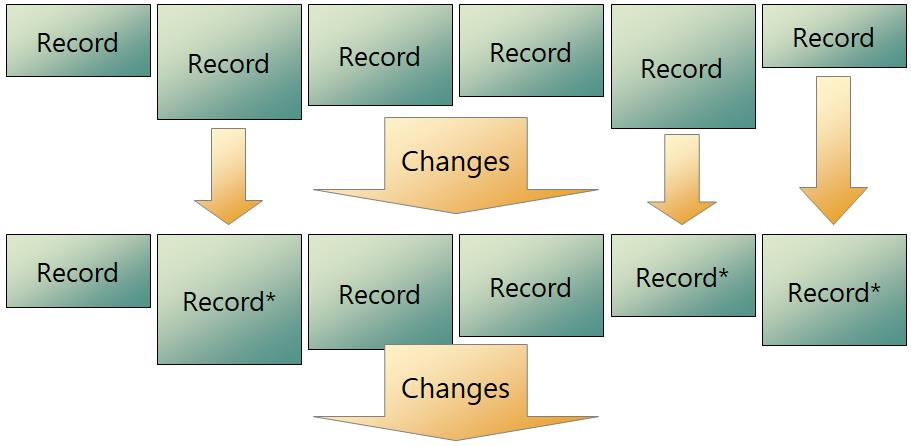
\includegraphics[width=0.9\textwidth]{content/1/chapter4/images/14.jpg}\\
Figure 4.14 – The record editing problem. In each change set, the records marked by * are edited, the rest remains unchanged
\end{center}

The most straightforward way to solve this problem is to store records in their own memory allocation and organize them in some data structure that allows each record to be replaced by a new one (the old record is deallocated, since the new one is, generally, of a different size). The data structure can be a tree (set in C++) or a list. To make the example more concrete, let us use strings for records. We also must be more specific about the way the change set is specified. Let us say that it does not point to a specific record that needs to be changed; instead, for any record, we can say whether it needs to be changed or not. The simplest example of such a change set for strings is a set of find and replace patterns. Now we can sketch our implementation:

\begin{lstlisting}[style=styleCXX]
std::list<std::string> data;
… initialize the records …
for (auto it = data.begin(), it0 = --data.end(), it1 = it;
true; it = it1) {
	it1 = it;
	++it1;
	const bool done = it == it0;
	if (must_change(*it)) {
		std::string new_str = change(*it);
		data.insert(it, new_str);
		data.erase(it);
	}
	if (done) break;
}
\end{lstlisting}

In every change set, we iterate over the entire collection of records, determine if the record needs to be changed, and, if needed, do so (the change set is hidden inside the functions must\_change() and change()). The code shows just one change set, so we run this loop as many times as needed.

The weakness of this algorithm is that we are using a list, and, to make it even worse, we keep moving the strings in memory. Every access to a new string is a cache miss. Now, if the strings are very long, then the initial cache miss doesn't matter, and the rest of the string is read using fast sequential access. The result is similar to the block-allocated array we saw earlier, and the memory performance is fine. But if the strings are short, the entire string may well be read in a single load operation, and every load is done at a random address.

Our entire algorithm does nothing but loads and stores at random addresses. As we have seen, this is pretty much the worst way to access memory. But what else can we do? We can't store the strings in one huge array: if one string in the middle of the array needs to grow, where would the memory come from? Right after that string is the next string, so there is no room to grow.

Coming up with an alternative requires a paradigm shift. The algorithm that performs the required operations literally as specified also imposes restrictions on the memory organization: changing records requires moving them in memory, and, as long as we want to be able to change any one record without affecting anything else, we cannot avoid random distribution of records in memory. We have to come at the problem sideways and start with the restrictions. We really want to access all records sequentially. What can we do under this constraint? We can read all records very fast. We can decide whether the record must be changed; this step is the same as before. But what do we do if the record must grow? We have to move it somewhere else, there is no room to grow in place. But we agreed that the records would remain allocated in sequence, one after the other. Then the previous record and the next record have to be moved too, so they remain stored before and after our new record. This is the key to the alternative algorithm: all records are moved with each change set, whether they are changed or not. Now we can store all records in one huge contiguous buffer (assuming we know the upper limit on the total record size):

\hspace*{\fill} \\ %插入空行
\begin{center}
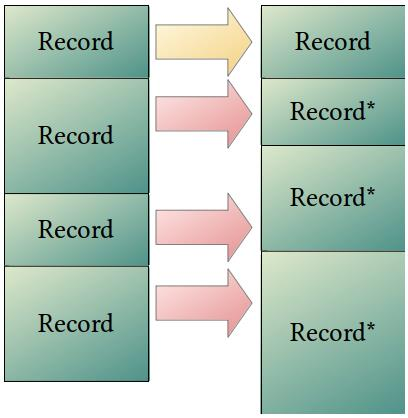
\includegraphics[width=0.9\textwidth]{content/1/chapter4/images/15.jpg}\\
Figure 4.15 – Processing all records sequentially
\end{center}

The algorithm requires allocating the second buffer of equal size during the copying, so the peak memory consumption is twice the size of the data:

\begin{lstlisting}[style=styleCXX]
char* buffer = get_huge_buffer();
… initialize N records …
char* new_buffer = get_huge_buffer();
const char* s = buffer;
char* s1 = new_buffer;
for (size_t i = 0; i < N; ++i) {
	if (must_change(s)) {
		s1 = change(s, s1);
	} else {
		const size_t ls = strlen(s) + 1;
		memcpy(s1, s, ls);
		s1 += ls;
	}
	s += ls;
}
release(buffer);
buffer = new_buffer;
\end{lstlisting}

In every change set, we copy every string (record) from the old buffer to the new one. If the record needs to be changed, the new version is written into the new buffer. Otherwise, the original is simply copied. With every new change set, we will create a new buffer and, at the end of the operation, release the old one (a practical implementation would avoid repeated calls to allocate and deallocate memory and simply swap two buffers).

The obvious downside to this implementation is the use of the huge buffer: we have to be pessimistic in choosing its size to allocate enough memory for the largest possible records we might encounter. Doubling of the peak memory size is also concerning. We can solve this problem by combining this approach with the growable array data structure we saw earlier. Instead of allocating one contiguous buffer, we can store the records in a series of fixed-size blocks:

\hspace*{\fill} \\ %插入空行
\begin{center}
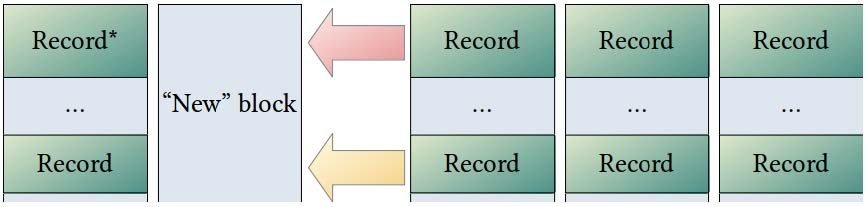
\includegraphics[width=0.9\textwidth]{content/1/chapter4/images/16.jpg}\\
Figure 4.16 – Using a block buffer to edit records
\end{center}

To simplify the diagram, we draw all records of the same size, but this restriction is not necessary: the records can span multiple blocks (we treat the blocks as a contiguous sequence of bytes, nothing more). When editing a record, we need to allocate a new block for the edited record. As soon as the editing is done, the block (or blocks) that contained the old record can be released; we don't have to wait for the entire buffer to be read. But we can do even better than that: instead of returning the recently freed block to the operating system, we can put it on the list of empty blocks. We are about to edit the next record, and we will need an empty new block for the result. We just happened to have one: it's the block that used to contain the last record we edited; it is at the head of our list of recently released blocks, and, best of all, that block is the last memory we accessed, so it is probably still in the cache!

At first glance, this algorithm seems a really bad idea: we are going to copy all the records every time. But let us analyze the two algorithms more carefully. First of all, the amount of reading is the same: both algorithms must read each string to determine whether it must be changed. The second algorithm is already ahead in performance: it reads all data in a single sequential sweep, while the first algorithm jumps around the memory. If the tring is edited, then both algorithms must write a new one into a new area of memory. The second algorithm again comes out ahead due to its sequential memory access pattern (also, it does not need to do a memory allocation for every string). The tradeoff comes when the string is not edited. The first algorithm does nothing; the second one makes a copy.

From this analysis, we can define the good and bad cases for each algorithm. The sequential access algorithm wins if the strings are short, and a large fraction of them are changed in every change set. The random access algorithm wins if the strings are long or if very few of them are changed. However, the only way to determine what is long and how many are a large fraction is to measure.

The fact that we must measure the performance does not necessarily mean that you have to always write two versions of the complete program. Very often, we can simulate the particular aspect of the behavior in a small mock program that operates on the simplified data. We just need to know the approximate size of the records, how many are changed, and we need the code that does the change to a single record so we can measure the impact of the memory accesses on performance (if each change is very computationally expensive, it won't matter how long it takes to read or write the record). With such mock or prototype implementation, we can do the approximate measurements and make the right design decision.

So, in real life, is the sequential string-copying algorithm ever worth it? We have done the tests for editing medium-length strings (128 bytes) using a regular expression pattern. If 99\% of all strings are edited in each change set, the sequential algorithm is approximately four times faster than random (the results will be somewhat specific to a machine, so the measurements must be done on the hardware similar to what you expect to use). If 50\% of all records are edited, the sequential access is still faster, but only by about 12\% (this is likely to be within the variation between different models of CPU and types of memory, so let's call it a tie). The more surprising result is that if only 1\% of all records are changed, the two algorithms are almost tied for speed: the time saved by not doing a random read pays for the cost of the almost entirely unnecessary copying.

For longer strings, the random-access algorithm wins handily if few strings are changed, and for very long strings, it's a tie even if all strings are changed: both algorithms read and write all strings sequentially (the random access to the beginning of a long string adds negligible time).

We now have everything we need to determine the better algorithm for our application. This is the way the design for performance often goes: we identify the root of the performance problem, we come up with a way to eliminate the issue, at the cost of doing something else, and then we have to hack together a prototype that lets us measure whether the clever trick actually pays off.

Before we end this chapter, I would like to show you an entirely different "use" of the performance improvements provided by the caches and other hardware.




























